%\part{Faire tourner le mod\`ele}


\chapter{Running the model: a practice simulation}

\label{loc:contact1}

This chapter is meant for first time users of the LMD model.
As the best introduction to the model is surely to run a simulation,
here we explain how to go about it.
All you will need are files and scripts necessary to build the GCM (all are in
the {\tt LMDZ.COMMON} and {\tt LMDZ.MARS} directories which you will download
as explained in the next
sections) as well as some initial states to initiate simulations and,
if not working on the
LMD machines, some extra datafiles for external forcings (topography,
dust scenarios, radiative properties of dust and water ice, etc.).\\
Once you have followed the example given below,
you can then go on to change the control parameters and the initial states
as you wish. A more detailed description of the model's organization
as well as associated inputs and
outputs are given in sections~\ref{sc:info} and~\ref{sc:io}.

\section{Obtaining the model}
The LMD model project is developped using subversion (svn), the free software
versioning and a revision control system.
To obtain (download) the latest version of the model,
simply go to the directory where you want to
install the model and use the relevant svn command:\\
{\tt svn checkout http://svn.lmd.jussieu.fr/Planeto/trunk --depth empty}\\
Then move to the newly generated {\tt trunk directory} and download
(i.e. {\tt svn update}) the
{\tt LMDZ.MARS} and {\tt LMDZ.COMMON} directories (the contents of these
directories are described in chapter \ref{loc:contenu}) with:
\begin{verbatim}
svn update LMDZ.MARS LMDZ.COMMON UTIL
\end{verbatim}

If you are not on the LMD machines, you will also need to download a
set of files available online at:\\
{\verb+http://www.lmd.jussieu.fr/~lmdz/planets/mars/datadir+}\\
(preserve the file names and subdirectory structure).
This directory contains input files (topography, dust scenarios,
radiative properties of scatteres, etc.) which the GCM needs to run.
Where you put your local {\tt datadir} directory (or whatever name
you choose for this directory) is not critical, as that location can
be specified at runtime (see sections \ref{sc:running_gcm} and
\ref{sc:callphys.def}).\\

To run the model, you will also need some initial condition files that
can be downloaded from:\\
{\verb+http://www.lmd.jussieu.fr/~lmdz/planets/mars/starts+}
(see section \ref{sc:inputfiles}).

\section{Prerequisites}
Before downloading and installing the model, a few prerequisites
must be satisfied:
\begin{enumerate}
\item The NetCDF library must be installed
 on your system, using the same
 compiler suite (e.g. gfortran and gcc, or ifort and icc) that you will use
 to compile the model. The latest version of the NetCDF package is available
 on the web at the following address:
  \begin{verbatim}
  http://www.unidata.ucar.edu/software/netcdf
  \end{verbatim}
  along with instructions for building (or downloading precompiled
  binaries of) the library.\\
  Note that we provide in the {\tt UTIL} directory a Bash script
  {\tt install\_netcdf4.0.1.bash} which may be used to download and install
  version 4.0.1 of the NetCDF library; run {\tt install\_netcdf4.0.1.bash -h}
  to list available options.
\item Some software to load and display NetCDF files such as 
   \begin{itemize}
   \item Ferret {\tt http://ferret.wrc.noaa.gov/Ferret}
   \item Panoply {\tt https://www.giss.nasa.gov/tools/panoply}
   \item GrAdS {\tt http://grads.iges.org/grads}
   \item ncview {\tt http://meteora.ucsd.edu/\~pierce/ncview\_home\_page.html}
   \end{itemize}
   among others, should be installed on your system.
\item The {\tt fcm} utility must be installed on your system.
  If it is not already so, it may be obtained by the following svn command:\\
  {\tt svn checkout http://forge.ipsl.jussieu.fr/fcm/svn/PATCHED/FCM\_V1.2}\\
  And add its {\tt bin} subdirectory to your {\tt PATH} environment variable
  to make the {\tt fcm} command available from anywhere.
\item To run at higher resolution (and/or with many tracers) requires some memory, in particular a reasonable stacksize (which is often quite limited by default). It is thus highly recommended that you set this value to {\tt unlimited} via
the command
\begin{verbatim}
ulimit -s unlimited
\end{verbatim}
before running the GCM, or more pragmatically by adding this instruction to you
{\tt .bashrc} or {\tt .profile} so that it is always set.
\end{enumerate}

\section{Installing the model}
Scripts for installation/compilation for the model are in the {\tt LMDZ.COMMON} directory
These scripts can also run the model on parallel computers. 

You should first compile the IOIPSL library which is used\footnote{It is in fact for now possible to run the GCM without the IOIPSL library but this requires adding the {\tt -io noioipsl} to the {\tt makelmdz\_fcm} command line, and might no longer be possible in the future.} by the GCM. To do this go to the {\tt LMDZ.COMMON/ioipsl} directory. There are a number of example scripts (depending on machines and compiler suites to use) to run to download and install the ioipsl library. As an illustrative example we detail here using the {\tt install\_ioipsl\_gfortran.bash} script:
\begin{itemize}
\item Edit script {\tt install\_ioipsl\_gfortran.bash} to set the path to your NetCDF library in the {\tt setfolder} variable, e.g. \verb+ setfolder="/usr/local/netcdf"+
\item Run the script: \verb+ ./install_ioipsl_gfortran.bash+
\item If all went well the script should end with the message \verb+ OK: ioipsl library is in + followed by the full path to the library {\tt libioipsl.a} and companion module files in in subdirectory \verb+modipsl/lib+
\end{itemize}

\section{Compiling the model}
\label{sc:compile}
The Bash script {\tt makelmdz\_fcm} is used to compile the model.
It needs not be modified or adapted to your settings, as all
specificities are set in corresponding files located in the {\tt arch}
subdirectory. For a given machine, e.g. {\tt MyMachine}, one should create
two files, {\tt arch-MyMachine.fcm} and {\tt arch-MyMachine.path}, using the
provided example files to set appropriate compiler options and paths
(for instance {\tt arch-linux-ifort-para.fcm} and
{\tt arch-linux-ifort-para.path} are adapted to run on local LMD machines).\\
The {\tt makelmdz\_fcm} script has the mandatory option {\tt -arch MyArch}
to specify the arch files to use (the {\tt "MyArch"} string should be replaced
with the name used for your own arch files), and multiple options:
\begin{itemize}
\item Example 1: Compiling the Martian model at grid resolution 64x48x49
\begin{verbatim}
makelmdz_fcm -arch linux-ifort -d 64x48x49 -p mars gcm
\end{verbatim}
\item Example 2: Compiling as above but in "debug" mode
\begin{verbatim}
makelmdz_fcm -arch linux-ifort -d 64x48x49 -p mars -debug gcm
\end{verbatim}
\item Example 3: Compiling the model to run in parallel (MPI) mode:
\begin{verbatim}
makelmdz_fcm -arch linux-ifort -parallel mpi -d 64x48x49 -p mars gcm
\end{verbatim}
This option is different from the -j option that determines the number of cores when compilation is run in parallel mode.
\item For an overview of all available options:
\begin{verbatim}
makelmdz_fcm -h
\end{verbatim}
\end{itemize}
Upon succesfull compilation, the GCM executable is generated in the
{\tt LMDZ.COMMON/bin} directory with the following naming convention:
\begin{verbatim}
gcm_XXX_phymars_YY.e
\end{verbatim}
where \verb+XXX+ is the model resolution (which was specified with the {\tt -d} argument) and \verb+YY+ is either \verb+seq+ or \verb+para+ depending on if the model was compiled in serial or parallel mode ({\tt -parallel} argument).

\section{Input files (initial states and def files)}
\label{sc:inputfiles}
In directory \verb+LMDZ.MARS/deftank+
you will find some examples of run
parameter files ({\tt .def} files) which the model needs at runtime.
The four files the model requires (they must be in the same directory as the
executable {\tt gcm.e}) are:
{\bf run.def} (described in 
section~\ref{loc:entrees}) {\bf callphys.def}
(see section~\ref{sc:callphys.def}), 
{\bf callphys.def}, {\bf z2sig.def} and {\bf traceur.def}.\\

The example {\tt .def} files given in the {\tt deftank} directory
are for various configurations (e.g. model resolution), copy (and eventually
rename these files to match the generic names) to the directory where
you will run the model.\\

Copy initial condition files
{\bf start.nc} and {startfi.nc}  (described in section
\ref{loc:entrees}) to the same directory.\\
You can extract such files from {\bf start\_archive}
`banks of initial states' (i.e. files which
contain collections of initial states from
stndard scenarios and which can thus be used
to check if the model is installed correctly) stored on the LMD website at
\verb+http://www.lmd.jussieu.fr/~lmdz/planets/mars/starts+.
See section~\ref{sc:newstart} for a description of how to proceed to
extract {\bf start} files from {\bf start\_archives}.

\section{Running the model}
\label{sc:running_gcm}
\begin{figure}
\centerline{\framebox[1.4\textwidth][c]{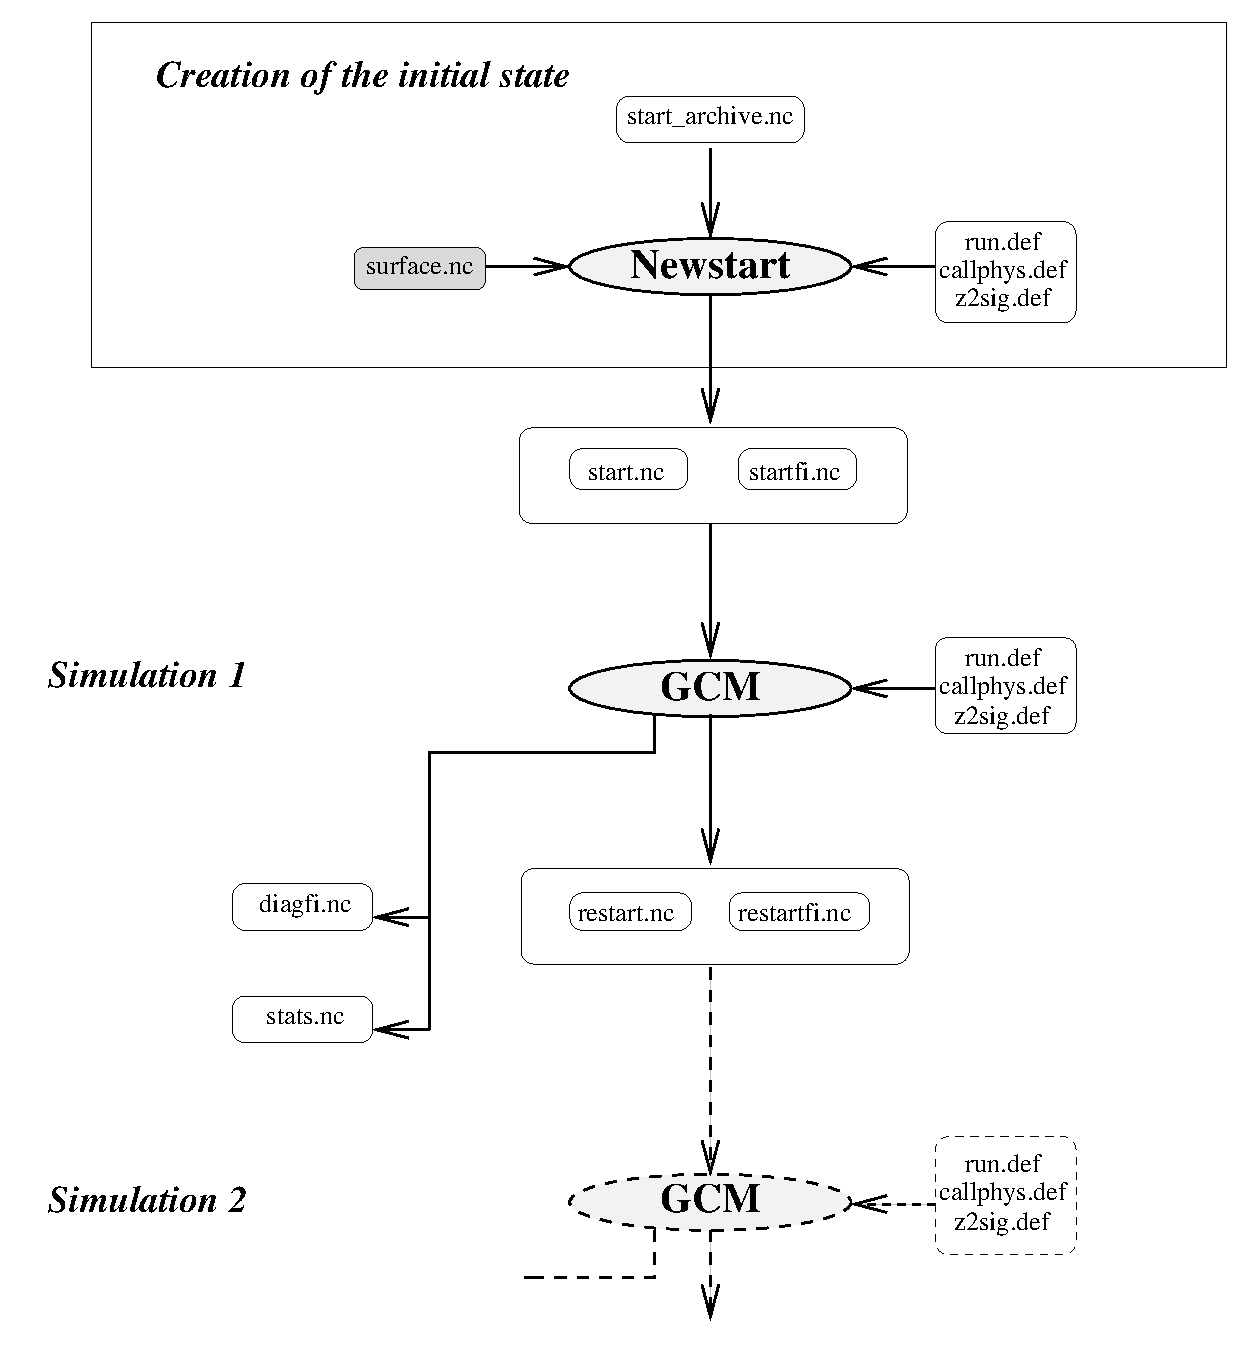
\includegraphics[width=1.2\textwidth]{Fig/inout.pdf}}}
\caption{Input/output data}
\label{fig:inout}
\end{figure}

Once you have the program {\bf gcm.e},
input files {\bf start.nc} {\bf startfi.nc},
and parameter files {\bf run.def callphys.def traceur.def z2sig.def}
in the same directory,
simply execute the program to run\footnote{
Note that if you ar not running on the LMD machines, you'll have to
modify or add, in file {\tt callphys.def}, the line:
{\tt datadir = /path/to/datafile}\\
Where {\tt /path/to/datafile} is the full path to the directory which
contains the set of files downloaded from:\\
\verb+http://www.lmd.jussieu.fr/~lmdz/planets/mars/datadir+
}
a simulation: 
\begin{verbatim}
gcm.e
\end{verbatim}

You might also want to keep all messages and diagnotics written to standard
output (i.e. the screen). You should then redirect the standard output
(and error) to some file, e.g. {\tt gcm.out}:
\begin{verbatim}
gcm.e > gcm.out 2>&1
\end{verbatim}

If you want to use parallel mode (as MPI for instance), you should specify it as follow:
\begin{verbatim}
mpirun gcm.e > gcm.out 2>&1
\end{verbatim}
NB: The definition of parallel parameters, such as number of cores, is dependant on the machine used.
You should find examples of scripts within other simulations or machine user guides.


\section{Visualizing the output files}

As the model runs it generates output files {\bf diagfi.nc} and
{\bf stats.nc} files. The former contains instantaneous values of
various fields and the later statistics (over the whole run) of some
variables.

\subsection{Using Ferret to visualize outputs}
Documentation and tutorials are available on the Ferret official website:
\begin{verbatim}
https://ferret.pmel.noaa.gov/Ferret/
\end{verbatim}
If you are a new user, we strongly recommend first spending some time browsing the official tutorials and documentation to learn more about Ferret capabilities and usage.\\

Here is asimple illustrative example of how one may visualize temperature for the 5th layer and 9th time step from a {\tt diagfi.nc} file:
\begin{description}
\item {\bf -} Ferret session:
  \begin{description}
  \item \verb+ferret+ {\it return}
  \item \verb!yes? use diagfi.nc!
  \item \verb!yes? show data! (displays information about available variables and their dimensions)
  \item \verb!yes? fill temp[k=5,l=9]! (plot temperature map of 5th layer and 9th time step) 
  \end{description}
\end{description}

\subsection{Using GrAds to visualize outputs}
If you have never used the graphic software {\bf GrAds}, we strongly
recommend spending half an hour to familiarize yourself with it by following
the demonstration provided for that purpose.
The demo is fast and easy to follow and you will learn the basic commands.
To do this read file 
\begin{verbatim}
/distrib/local/grads/sample
\end{verbatim}

For example, to visualize files {\tt diagfi.nc} and {\tt stats.nc}

NetCDF files {\tt diagfi.nc} and {\tt stats.nc} can be accessed directly
using GrAdS thanks to utility program gradsnc,
(the user does not need to intervene).\\

\noindent
To visualize the temperature in the 5th layer using file
{\tt diagfi.nc} for example:
\label{loc:visu}

\begin{description}
\item {\bf -} GrAdS session:

  \begin{description}
  \item \verb+grads+ {\it return}

  \item {\it return} (opens a landscape window)

  \item \verb+ga-> sdfopen diagfi.nc+ 

  \item \verb+ga-> query file+ (displays info about the open file, including the name of the stored variables. Shortcut: {\it q file})

  \item \verb+ga-> set z 5+ (fixes the altitude to the 5th layer)

  \item \verb+ga-> set t 1+ (fixes the time to the first stored value)

  \item \verb+ga-> query dims+ (indicates the fixed values for the 4
  dimensions. Shortcut: {\it q dims})

  \item \verb+ga-> display temp+ (displays the temperature card for the 5th layer and for the first time value stored. Shortcut: {\it d
  T})

  \item \verb+ga-> clear+ (clears the display. Shortcut: {\it c})

  \item \verb+ga-> set gxout shaded+ (not a contour plot, but a shaded one)

  \item \verb+ga-> display temp+ 

  \item \verb+ga-> set gxout contour+ (returns to contour mode to display the levels)

  \item \verb+ga-> display temp+ (superimposes the contours if the clear command is not used)

  \end{description}
\end{description}



%%%%%%%%%%%%%%%%%%%%%%%%%%%%%%%%%%%%%%%%%%%%%%%%%%%%%%%%%%%%%%%%%%%%%%%

\section{Resuming a simulation}
At the end of a simulation, the model generates {\bf restart} files
(files {\tt restart.nc} and {\tt restartfi.nc})
which contain the final state of the model.
As shown in figure~\ref{fig:inout},
these files (which are of the same format as the start files)
can later be used as initial
states for a new simulation.\\

\noindent
The {\bf restart} files just need to be renamed:
\begin{verbatim} 
mv restart.nc start.nc
mv restartfi.nc startfi.nc
\end{verbatim}
\noindent
and running a simulation with these will in fact resume the simulation
from where the previous run ended.

\section{Chain simulations}

In practice, we recommend running a chain of simulations lasting several
days or longer (or hundreds of days at low resolution).

To do this, a script named {\tt run0} is available in
\verb+LMDZ.MARS/deftank+ , which should be used as follows:
\begin{itemize}
\item Set the length of each simulation in {\tt run.def}
 (i.e. set the value of {\tt nday})
\item Set the maximum number of simulations at the beginning of the {\tt run0}
script (i.e. set the value of {\tt nummax})
\item Copy start files {\tt start.nc  startfi.nc} over and rename them
      {\tt start0.nc startfi0.nc}.
\item Run script {\tt run0} 
\end{itemize}

{\tt run0} runs a series of simulations that generate the indexed output
files (e.g. {\tt start1, startfi1, diagfi1}, etc.)
including files {\tt lrun1, lrun2}, etc. containing the redirection of the
display and the information about the run. 

{\it NOTE:} to restart a series of simulations after a first series
(for example, starting from {\tt start5 and  startfi5}), just write the
index of the initial files (e.g. 5) in the file named {\tt num\_run}.
If {\tt num\_run} exists, the model will start from the index written in
{\tt num\_run}. If not it will start from, {\tt start0 and startfi0}.


{\it NOTE}: A script is available for performing annual runs with 12 seasons
at 30$^o$ solar longitude
as it is in the database (script {\bf \tt run\_mcd}, also found in directory
{\tt deftank}).
This script functions with script run0. Just set the number of simulations to
1 in run0. Then copy run.def into run.def.ref and set nday to 9999 in this
file. To start from startN.c, edit the file run\_mcd and comment
(with a \#) the N months already created and describe N in {\tt num\_run}. 
Then run  {\bf \tt run\_mcd}.


\section{Creating and modifying initial states}

\label{sc:newstart}

\subsection{Using program ``newstart''}

Several model parameters (for example, the dust optical depth) are stored in
the initial states (NetCDF files {\tt start.nc}
and {\tt startfi.nc}).
To change these parameters, or to generally change the model resolution,
use program {\bf newstart}.

This program is also used to create an initial state.
In practice, we usually reuse an old initial state, and modify it using
{\bf newstart}.

Like the GCM, program {\bf newstart} must be
compiled (using the {\tt makelmdz\_fcm} script)
at the required grid resolution.
For example:
\begin{verbatim}
makelmdz_fcm -arch local -d 64x48x25 -p mars newstart
\end{verbatim}
The resulting executable will be created in the {\tt LMDZ.COMMON/bin} directory, as \verb+newstart_XXX_phymars_seq.e+, where \verb+XXX+ is the dimension (values given to the {\tt -d} argument) for which newstart was compiled.\\

Then run the newstart program in a directory containing the start
and def file to be used:
\begin{verbatim}
newstart.e
\end{verbatim}

The program then gives you two options:
\begin{verbatim}
 From which kind of files do you want to create newstart and startfi files
     0 - from a file start_archive
     1 - from files start and startfi
\end{verbatim}

\begin{itemize}
\item{-} Option ``1'' allows you to read and modify the information needed
to create a new initial state  from the files
\verb+ start.nc, startfi.nc + 
\item{-} Option ``0'' allows you to read and modify the information needed to
create a new initial state from file
\verb+ start_archive.nc + (whatever the \verb+ start_archive.nc +
grid resolution is).\\
\end{itemize} 
If you use tracers, make sure that they are taken into account in your
start files (either start or start\_archive).\\ \\
Then answer to the various questions in the scroll menu.
These questions allow you to modify the initial state for the following
parameters. 

{\footnotesize
\begin{verbatim}
 First set of questions:
 Change values in tab_cntrl ? :
 ~~~~~~~~~~~~~~~~~~~~~~~~~~~~~~
 (Current values given above)

 (3)          day_ini : Initial day (=0 at Ls=0)
 (19)              z0 :  surface roughness (m)
 (21)       emin_turb :  minimal energy (PBL)
 (20)         lmixmin : mixing length (PBL)
 (26)         emissiv : ground emissivity
 (24 et 25)   emisice : CO2 ice max emissivity
 (22 et 23)  albedice : CO2 ice cap albedos
 (31 et 32) iceradius : mean scat radius of CO2 snow
 (33 et 34) dtemisice : time scale for snow metamorphism
 (27)        tauvis : mean dust vis. reference opacity
 (35)      volcapa : soil volumetric heat capacity
 (18)     obliquit : planet obliquity (deg)
 (17)     peri_day : periastron date (sols since Ls=0)
 (15)     periastr : min. star-planet dist (Mkm)
 (16)     apoastr  : max. star-planet (Mkm)
 (14)     year_day : length of year (in sols)
 (5) rad : radius of the planet (m)
 (6) omeg : planet rotation rate (rad/s)
 (7) g : gravity (m/s2)
 (8) mugaz : molecular mass of the atmosphere (g/mol)
 (9) rcp : r/Cp
 (10) daysec : length of a sol (s)

 Second set of questions :
 flat : no topography ("aquaplanet")
 bilball : uniform albedo and thermal inertia
 coldspole : cold subsurface and high albedo at S.pole
 qname : change tracer name
 q=0 : ALL tracer =zero
 q=x : give a specific uniform value to one tracer
 ini_q : tracers initialisation for chemistry, water and ice
 ini_q-H2O : tracers initialisation for chemistry and ice
 ini_q-iceH2O : tracers initialisation for chemistry only
 noglacier : Remove tropical H2O ice if |lat|<45
 watercapn : H20 ice on permanent N polar cap
 watercaps : H20 ice on permanent S polar cap
 oborealis : H2O ice across Vastitas Borealis
 iceball   : Thick ice layer all over surface
 wetstart  : start with a wet atmosphere
 isotherm  : Isothermal Temperatures, wind set to zero
 radequi   : Earth-like rad. eq. temperature profile and winds set to zero
 co2ice=0 : remove CO2 polar cap
 ptot : change total pressure
 emis : change surface emissivity
 therm_ini_s : Set soil thermal inertia to reference suface values
\end{verbatim}
}
 

Program {\bf newstart.e} creates files 
{\tt restart.nc} and {\tt restartfi.nc}
that you generally need to rename (for instance rename them in start0.nc
and startfi0.nc if you want to use run0 or run\_mcd, starting with season 0;
rename them {\tt start.nc} and {\tt startfi.nc} if you just want to perform
one run with {\tt gcm.e}). 


\subsection{Creating the initial start\_archive.nc file } 

Archive file
{\tt start\_archive.nc} is created from files
{\tt start.nc} and {\tt startfi.nc} by program {\bf start2archive}.
Program {\bf start2archive} compiles to the same grid resolution as the
{\tt start.nc} and {\tt startfi.nc} grid resolution. For example:

\begin{verbatim}
makelmd_fcm -arch local -d 64x48x25 -p mars start2archive
\end{verbatim}
Then run \verb+ start2archive.e+ \\ \\
You now have a \verb+ start_archive.nc+ file for one season that you can
use with newstart.
If you want to gather other states obtained at other times of year, rerun
{\tt start2archive.e} with the {\tt start.nc} and {\tt startfi.nc}
 corresponding to these.
These additional initial states will automatically be added to the
{\tt start\_archive.nc} file present in the directory.  

\subsection{Changing the horizontal or vertical grid resolution}

To run at a different grid resolution than available initial conditions
files, one needs to use tools {\bf newstart} and {\bf start2archive}

For example, to create initial states at grid resolution
32$\times$24$\times$25 from NetCDF files
\verb+ start + and \verb+ startfi + at grid resolution
  64$\times$48$\times$32 :

\begin{itemize}
\item Create file \verb+ start_archive.nc + 
with {\bf start2archive.e} compiled at grid resolution
64$\times$48$\times$25 using {\bf old file {\tt z2sig.def}
 used previously}

\item Create files 
{\tt newstart.nc} and {\tt newstartfi.nc}
 with {\bf newstart.e}
compiled at grid resolution 32$\times$24$\times$25,
using {\bf new file {\tt z2sig.def}}

\end{itemize} 

If you want to create starts files with tarcers for 49 layers using a
{\tt start\_archive.nc} obtained for 32 layers, do not forget to use the
\verb+ ini_q+ option in newstart in order to correctly initialize tracers
value for layer 33 to layer 49.
You just have to answer yes to the question on thermosphere initialization
if you want to initialize the thermosphere part only (l=33 to l=49),
and no if you want to initialize tracers for all layers (l=0 to l=49).\\ \\

